\section{Theoretical Analysis}
\label{sec:analysis}

In this section, we used the theorectical model as presented in the lectures. To do so we adopted the equations provided in lecture 16 and 17 and utilised the values of the circuit parameters, that we optimized with the help of Ngspice tool, as showcased previously.

The circuit was divided in two main parts, the gain and output stages. These were combined together because they complemented one another.

The gain stage which consists of a common emitter amplifier has the advantage of generating a high, desirable gain. However, along with this comes the cost of having a very high output impedance which squanders the gain.

\begin{table}[h]
  \centering
  \begin{tabular}{|l|r|}
    \hline    
    {\bf Parameters} & {\bf Values} \\ \hline
    |VT| & 0.025000 \\ \hline
|beta| & 178.700000 \\ \hline
|VA| & 69.700000 \\ \hline
|VBEON| & 0.700000 \\ \hline
|Vcc| & 12.000000 \\ \hline
|Req| & 8461.538462 \\ \hline
|Veq| & 1.846154 \\ \hline
|IB1| & 0.000026 \\ \hline
|IC1| & 0.004613 \\ \hline
|IE1| & 0.004639 \\ \hline
 |$V_{emit}$| & 0.927733 \\ \hline
|$V_{coll}$| & 6.925864  \\ \hline
|VCE| & 5.998131 \\ \hline|$V_{base}$| & 1.627733  \\ \hline
  \end{tabular}
  \caption{Transistor`s parameters.}
  \label{tab:1}
\end{table}

\begin{table}[h]
  \centering
  \begin{tabular}{|l|r|}
    \hline    
    {\bf Parameters} & {\bf Values} \\ \hline
    |gm1| & 0.184514 \\ \hline
|ro1| & 15109.960453 \\ \hline
|rpi| & 968.489933 \\ \hline
  \end{tabular}
  \caption{Parameters of slide 10, lecture 16.}
  \label{tab:2}
\end{table}

\begin{table}[h]
  \centering
  \begin{tabular}{|l|r|}
    \hline    
    {\bf Parameters} & {\bf Values} \\ \hline
    |Input impedance| & 869.023345 \\ \hline
|Output impedance| & 1025.354537 \\ \hline
|Gain| & 169.668298 \\ \hline
|Gain(dB)| & 44.592014 \\ \hline
  \end{tabular}
  \caption{Gain and impedances.}
  \label{tab:3}
\end{table}


In order to reduce the high impedance value that is associated with the gain stage, we developed an output stage that allows to rectify the problem we had previously. Once again, we followed the instructions given in the lectures.

\begin{table}[h]
  \centering
  \begin{tabular}{|l|r|}
    \hline    
    {\bf Parameters} & {\bf Values} \\ \hline
    |VO2| & 7.625864 \\ \hline
|$V_{coll}$| & 6.925864 \\ \hline
|VA| & 7.625864 \\ \hline
|$V_{emit}$| & 12.000000 \\ \hline
|Vcc| & 0.000087 \\ \hline
|IB2| & 0.019795 \\ \hline
|IC2| & 0.019882 \\ \hline
|IE2| & 
  \end{tabular}
  \caption{Parameter values for the output stage.}
  \label{tab:4}
\end{table}

\begin{table}[h]
  \centering
  \begin{tabular}{|l|r|}
    \hline    
    {\bf Parameters} & {\bf Values} \\ \hline
    |gm2| & 0.791814 \\ \hline
|go2| & 0.000532 \\ \hline
|gpi2| & 0.003484 \\ \hline
|ge2| & 0.004545 \\ \hline
|Input Impedance| & 26837.230759 \\ \hline
|Output Impedance| & 1.249414 \\ \hline
|Gain| & 0.989304 \\ \hline
|Gain(dB)| & -0.093408 \\ \hline
  \end{tabular}
  \caption{Output stage impedance and gain.}
  \label{tab:5}
\end{table}

Finally, the gain results of the total circuit.

\begin{figure}[h] \centering
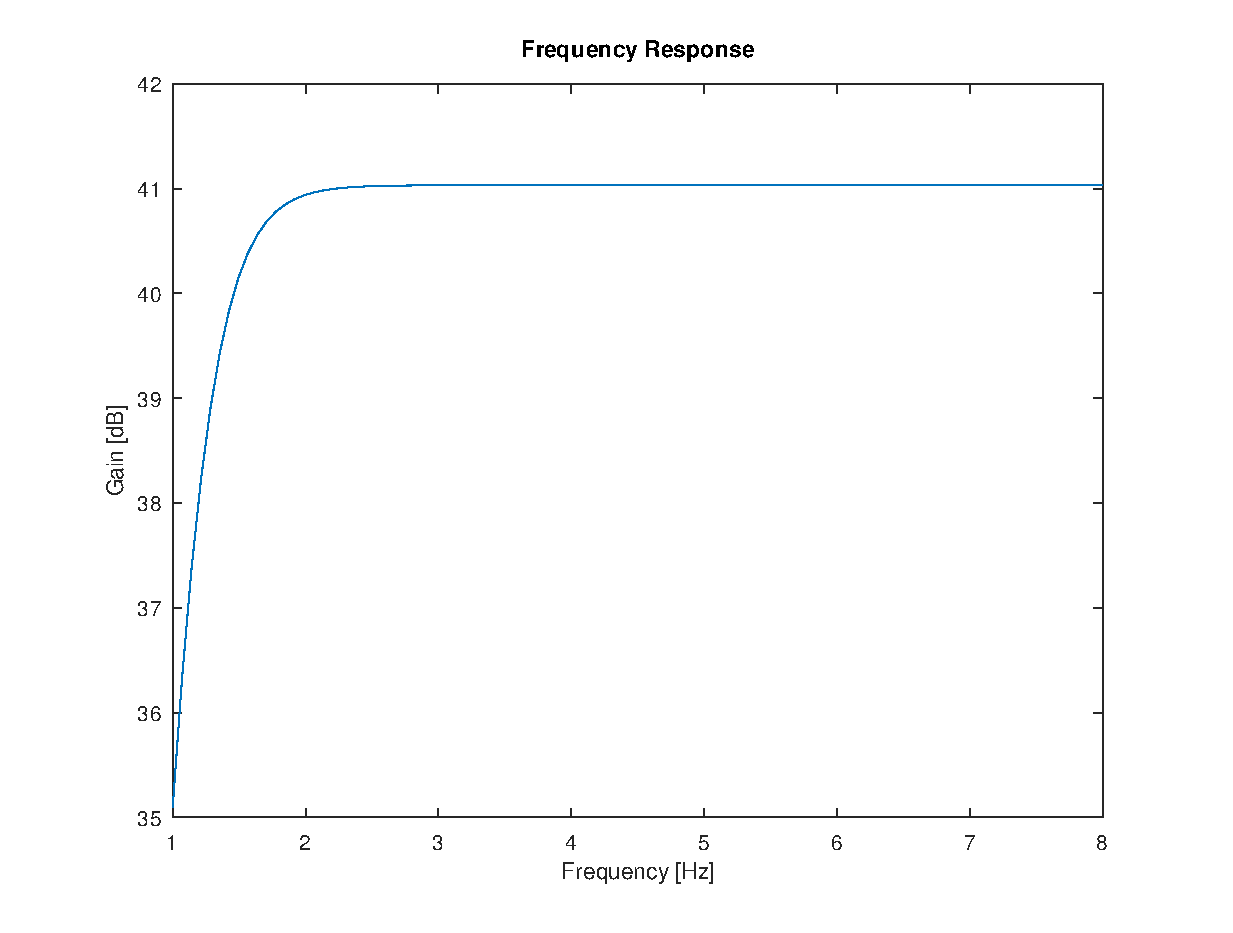
\includegraphics[width=0.6\linewidth]{freqresponse.eps}
\caption{Plot of Gain in order of the Frequency (Hz).}
\label{fig:plotA1}
\end{figure}
